\documentclass[12pt]{article}
\usepackage[utf8]{inputenc}
\usepackage[T2A]{fontenc}
\usepackage[russian, english]{babel}
\usepackage{amsmath,amssymb,amsfonts,mathtext,tikz}
\usepackage{graphicx}
\usepackage{booktabs}
\usepackage{hyperref}
\usepackage[most]{tcolorbox}
\usepackage{tabularx}
\usepackage{float}
\usepackage[style=verbose-ibid,backend=biber]{biblatex}
\addbibresource{references.bib}

% Настройка полей
\usepackage[margin=2.5cm]{geometry}

% Колонтитулы
\usepackage{fancyhdr}
\pagestyle{fancy}
\fancyhf{}
\fancyhead[L]{Инструменты разделения редких ресурсов}
\fancyhead[R]{25 мин}
\fancyfoot[C]{\thepage}
\renewcommand{\headrulewidth}{0.4pt}

% Цвета для блоков
\usepackage{xcolor}
\definecolor{blockblue}{RGB}{204,229,255}
\definecolor{blockred}{RGB}{255,229,204}

\title{\textbf{Инструменты разделения редких и неравномерно распределённых ресурсов}}
\author{}
\date{}

\begin{document}
\maketitle
\thispagestyle{fancy}

% ================= РАЗДЕЛ 1 — ВВЕДЕНИЕ: ПРОИЗВОДНЫЙ СПРОС =================
\section{Введение: почему это не про «рынок или государство»}

Население хочет \textbf{тепло}, а не нефть. Спрос на нефть — \emph{производный}:
\begin{equation}\label{eq:derived}
D_{oil}(p) = \sum_{i=1}^{n} \alpha_i D_i(p_i),
\end{equation}
где $\alpha_i$ — доля нефти в производстве блага $i$ (транспорт, свет, отопление, промышленность).

\textbf{Конкуренция} за ресурс идёт не на уровне домохозяйств, а на уровне:
\begin{itemize}
\item фирм (НПЗ, трейдеры, агроэкспорт),
\item государств (права на добычу, концессии, трансграничные воды).
\end{itemize}

Отсюда \textbf{ложная развилка}: «рынок или государство». Инструментарий шире — и сегодня мы инвентаризируем его как инженеры: без оценок, через параметры.

% ================= РАЗДЕЛ 2 — ТРИ ОСИ =================
\section{Три оси — не путать}

Три понятия, которые в бытовой речи сливаются, — \textbf{ограниченность}, \textbf{редкость}, \textbf{неравномерность} — имеют разную природу и требуют разных инструментов.

\subsection{Ограниченность (flow / stock)}
Физический/технический факт: \emph{потоковый} ресурс $\dot{Q} \le R$, \emph{запасовый} — $Q_{total} \le S$.

\textbf{Индикатор:} горизонт исчерпания $R/Q$ (для нефти — ~50 лет при текущем потреблении).

\textbf{Важный переход:} если $R/Q \to \infty$ (поток), но $S(0) \le 0$ (нет избыточного спроса при нулевой цене) — \emph{инструменты распределения не нужны}.

\subsection{Редкость (scarcity)}
Экономическое понятие: $S = D(0) - Q$ — избыточный спрос при нулевой цене.

\textbf{Параметры:}
\begin{itemize}
\item эластичность предложения (если $\eta \to \infty$ — редкость не растёт при росте спроса),
\item наличие положительной экономической ренты в цене,
\item отношение запасы/добыча (грубый индикатор).
\end{itemize}

\textbf{Пример:} воздух в чистом месте — $S(0) \le 0$ — не редок; воздух в мегаполисе — $S(0) > 0$ — редок.

\subsection{Неравномерность}
\textbf{Не то же, что редкость}. Это про «где ресурс находится и у кого права».

Три параметра разной природы:
\begin{enumerate}
\item \textbf{Геологическая концентрация} — доля мировых запасов в топ-$N$ странах (кобальт — ДР Конго, литий — литиевый треугольник).
\item \textbf{Институциональная концентрация} — концентрация прав (HHI по держателям лицензий). Именно она — в центре сюжета Перкинса: не «нефти нет у населения», а «права на нефть не у населения».
\item \textbf{Неравномерность доступа по покупательной способности} — даже при глобально достаточном объёме. Сен: голод — не от нехватки еды, а от краха entitlement.
\end{enumerate}

% ================= РАЗДЕЛ 3 — МАТРИЦА =================
\section{Матрица исключаемость / соперничество}

\begin{figure}[h]
\centering
\begin{tikzpicture}[scale=0.9]
\draw[->] (0,0) -- (6,0) node[right] {Исключаемость};
\draw[->] (0,0) -- (0,5) node[above] {Соперничество};
\draw[thick] (0,0) rectangle (3,3) node[midway] {Частные};
\draw[thick] (3,0) rectangle (6,3) node[midway] {Клубные};
\draw[thick] (0,3) rectangle (3,6) node[midway] {Общие (commons)};
\draw[thick] (3,3) rectangle (6,6) node[midway] {Открытый доступ};
\node at (1.5,1.5) {рынок};
\node at (4.5,1.5) {рынок / гос.};
\node at (1.5,4.5) {общинные правила};
\node at (4.5,4.5) {деградация};
\end{tikzpicture}
\caption{Четыре типа благ — разные инструменты}
\end{figure}

\textbf{Ключевой вывод:} сам по себе факт, что ресурс «общий», ещё не означает трагедии — нужен \textbf{режим собственности} (Остром, 1990).

% ================= РАЗДЕЛ 4 — ИНСТРУМЕНТАРИЙ (3 БЛОКА) =================
\section{Инструментарий — три блока}

\subsection{Блок 1. Режимы собственности}
\begin{itemize}
\item \textbf{Частная} — спецификация прав, можно продать (ITQ в Исландии).
\item \textbf{Государственная} — концессии, лицензии, государственная собственность на недра (Россия, США — federal lands).
\item \textbf{Общая (commons)} — правила сообщества, исключение чужих (huertas Валенсии, японские сатояма).
\item \textbf{Открытый доступ} — \emph{не является институтом}, это отсутствие режима.
\end{itemize}

\textbf{Важно:} реальные системы — гибриды. Рыболовные квоты — государственная собственность + временное частное право + перепродажа.

\subsection{Блок 2. Механизмы распределения}
\textbf{Рыночные:}
\begin{itemize}
\item аукцион (английский, голландский, Vickrey — доминирующая стратегия),
\item переуступаемые квоты (ITQ, cap-and-trade).
\end{itemize}

\textbf{Административные:}
\begin{itemize}
\item нормирование (паёк — Кейптаун 2018),
\item очередь (советская медицина — \emph{first-come-first-served}),
\item лотерея (green card, охота на лося),
\item административное распределение (UNOS — совместимость + ожидание + тяжесть).
\end{itemize}

\textbf{Гибрид:} ITQ — государство устанавливает $\sum E_i = E_{cap}$, затем права торгуются.

\subsection{Блок 3. Механизмы ограничения}
Два подхода — Пигу vs Коуз.

\textbf{Пигу:} обложить использование налогом = предельный внешний эффект (углеродный налог Швеции, Канады).

\textbf{Коуз:} чёткие права + рынок (cap-and-trade — $\text{SO}_2$ в США, EU ETS).

\textbf{Command-and-control:}
\begin{itemize}
\item технологические стандарты (катализаторы),
\item абсолютные лимиты (квоты ОПЕК+, квоты вылова ИКЕС),
\item зонирование,
\item концессии с условиями,
\item ротация (севооборот, пастбища).
\end{itemize}

\textbf{Правила самоуправления (Остром):} 8 условий — границы, правила под местные условия, коллективные решения, мониторинг, санкции, механизмы разрешения конфликтов, признание государством, вложенность.

% ================= РАЗДЕЛ 5 — КЕЙС: ВОДА (ЧИЛИ/АВСТРАЛИЯ) =================
\section{Кейс: вода — Чили (1981) vs Австралия (Murray--Darling)}

\subsection{Чили — Water Code 1981}
\begin{itemize}
\item Права — отделены от земли, бессрочны, торгуемы \cite{bauer2004chile}.
\item \textbf{Нет потолка} на изъятие по бассейнам.
\item Результат: концентрация прав (агроэкспорт), падение стока нижнего течения р. Петорка до \textbf{50\%} в засуху (DGA, 2015–2020) \cite{budds2008water}.
\end{itemize}

\subsection{Австралия — Cap-and-Trade (с 1995, план 2012)}
\begin{itemize}
\item $\bar{Q}$ — экологически устойчивый объём (определяется гидрологически).
\item $q_i = e_i \cdot \frac{\bar{Q}}{\sum e_i}$ — торговля \emph{долями} потолка.
\item Результат: засуха 2000–2008 — цена allocation выросла втрое, \textbf{но объём $\le \bar{Q}$}; сельхозпроизводство потеряло <1\% \cite{grafton2012water}.
\end{itemize}

\textbf{Формальная разница}

\vspace{0.3cm} % Небольшой отступ перед таблицей

\begin{tabular}{p{0.45\textwidth} p{0.45\textwidth}}
% Левая колонка (ширина 45% текста)
\textbf{Чили:}
$$q_i \ge 0,\quad \sum q_i \text{ не ограничен}$$
Цена $\to$ предельные издержки добычи.

\vspace{0.2cm} % Отступ между пунктами внутри ячейки

\textit{Результат:} концентрация прав, падение стока нижнего течения р. Петорка до \textbf{50\%} в засуху.
&
% Правая колонка (ширина 45% текста)
\textbf{Австралия:}
$$\bar{Q} = \sum q_i,\quad q_i = e_i \cdot \frac{\bar{Q}}{\sum e_i}$$
Цена — рента за долю потолка.

\vspace{0.2cm}

\textit{Результат:} засуха 2000–2008 — цена выросла втрое, но объём $\le \bar{Q}$; сельхозпроизводство потеряло $<1$\%.
\end{tabular}

\textbf{Одна и та же конструкция (торгуемые права) $\Rightarrow$ противоположные результаты.}

% ================= РАЗДЕЛ 6 — ВАЙЦМАН (ЦЕНА vs КОЛИЧЕСТВО) =================
\section{Правило Вайцмана (1974): цена vs количество}

\subsection{Модель}
Регулятор выбирает между:
\begin{itemize}
\item \textbf{ценой} (налог) — $p$ фиксирована, $q$ подстраивается,
\item \textbf{количеством} (квота) — $\bar{q}$ фиксирована, $p$ подстраивается.
\end{itemize}

При квадратичных функциях потерь и сдвиге $MC$:
\begin{equation}\label{eq:weitzman}
\frac{L_{\text{price}}}{L_{\text{quota}}} = \left( \frac{e}{f} \right)^2,
\end{equation}
где $e$ — наклон $MB$, $f$ — наклон $MC$.

\subsection{Интерпретация}
\begin{itemize}
\item $e < f$ (MB пологая) $\Rightarrow$ \textbf{налог} точнее.
\item $e > f$ (MB крутая) $\Rightarrow$ \textbf{квота} точнее.
\item «Толстые хвосты» (Weitzman 2009) — если рядом климатический порог — \textbf{квота}.
\end{itemize}

\subsection{Иллюстрация: углерод (Nordhaus 2018)}
\begin{figure}[h]
\centering
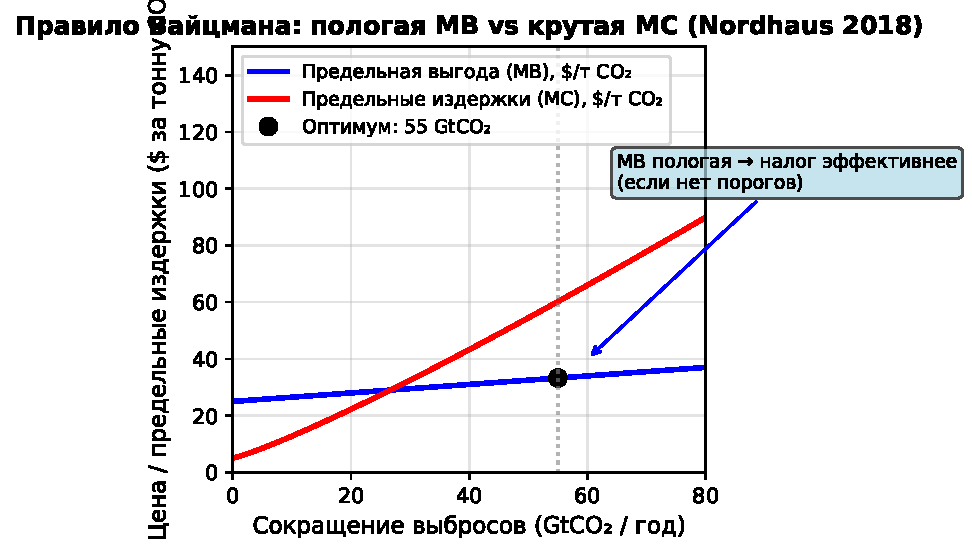
\includegraphics[width=0.9\linewidth]{nordhaus_mb_mc.pdf}
\caption{MB — пологая (предотвращённый ущерб), MC — крутая (цена декарбонизации). Оптимум ~55 $\text{GtCO}_2$/год, цена ~\$50–60/т. \cite{nordhaus2018soccost}}
\end{figure}

\textbf{Вывод для углерода:} при текущих оценках $e/f < 1$ — налог эффективнее. При крутых $MB$ (рядом с порогом) — квота.

% ================= РАЗДЕЛ 7 — UNOS: ТРЕТИЙ ПОЛЮС =================
\section{UNOS — третий полюс: приоритизация без денег}

\subsection{MELD 3.0 (2023) — распределение печени}
Компоненты балла:
\begin{itemize}
\item билирубин (лог), МНО (лог), креатинин (лог) + диализ,
\item пол: женщина $+1.33$ (коррекция систематического занижения),
\item исключения: гепатоцеллюлярная карцинома (HCC).
\end{itemize}

\subsection{Непрерывное распределение (2021--2023)}
\begin{itemize}
\item убраны границы Donor Service Area (DSA),
\item расстояние от донора — компонент балла,
\item баланс: \textbf{срочность} vs \textbf{пост-трансплантационная выживаемость}.
\end{itemize}

\textbf{Инструмент — не рынок, не государство, а \emph{механизм приоритизации} (балл).}

% ================= РАЗДЕЛ 8 — ДОПОЛНИТЕЛЬНЫЕ ПРИМЕРЫ (КРАТКО) =================
\section{Другие механизмы «эгоизма во вред себе»}

\subsection{Устойчивость к антибиотикам (flow, не stock)}
Общий ресурс — \textbf{эффективность класса препаратов}. Каждый врач получает 100\% пользы сейчас, издержки — на общество. Аналог — формула «трагедии общин» (Hardin, но для антибиотиков).

\subsection{Парадокс Браесса (congestion без истощения)}
Добавление дороги $\Rightarrow$ рост времени в пути. Каждый эгоистично выбирает «кратчайший» маршрут — итог хуже. \textbf{Инструмент:} плата за въезд (congestion pricing) — не квота.

\subsection{Банковская паника (игра без ресурса)}
Нет ресурса — есть структура ожиданий. Рациональный вкладчик бежит — банк рушится. \textbf{Инструмент:} страхование вкладов (FDIC) — не цена, не количество, а \textbf{институциональная гарантия}.

\subsection{Монголия — пастбища (commons $\to$ open access)}
\begin{itemize}
\item 1990-е — приватизация скота, земля — государственная,
\item общины потеряли контроль,
\item поголовье: $\sim 25 \to 47$ млн (1990--2010),
\item $70$--$88\%$ пастбищ деградированы (World Bank / FAO) \cite{worldbank2022mongolia}.
\end{itemize}
\textbf{Провал:} не отсутствие правил, а \textbf{разрушение работавшего института} без замены.

% ================= РАЗДЕЛ 9 — СИНТЕЗ =================
\section{Синтез: какой инструмент — когда?}

\begin{tabular}{@{}lll@{}}
\toprule
\textbf{Режим} & \textbf{Инструмент} & \textbf{Условие} \\
\midrule
Частная & Рынок & Спецификация прав \\
Государственная & Cap + trade & Измеримый потолок \\
Commons & Правила сообщества & Границы + мониторинг \\
Открытый доступ & — & Не является институтом \\
\bottomrule
\end{tabular}
\vspace{0.5cm}

\textbf{Общий принцип:} \\
\textit{Инструмент не выбирается — он следует из того, какой параметр вы можете измерить и удержать.}

\textbf{Примеры из доклада:}
\begin{itemize}
\item вода (Чили) — рынок (нет потолка),
\item вода (Австралия) — cap + trade (есть потолок),
\item углерод — Вайцман ($e < f$ — налог; рядом порог — квота),
\item органы — UNOS (приоритизация, не рынок).
\end{itemize}

% ================= РАЗДЕЛ 10 — ВОПРОС ЗАЛУ =================
\section{Вопрос залу}

На каком ресурсе из перечисленных вы бы \textbf{запретили} цену?
\begin{itemize}
\item вода,
\item органы,
\item радиочастоты,
\item углерод,
\item земля.
\end{itemize}

\vspace{1cm}
\begin{tcolorbox}{Основные источники}
Bauer (2004), Budds (2008), Grafton et al. (2012), Weitzman (1974), Nordhaus (2018), UNOS/OPTN Policy 4.0 (2023).
\end{tcolorbox}

% ================= РАЗДЕЛ 11 — АНАЛИЗ КНИГИ ДЖОНА ПЕРКИНСА "ИСПОВЕДЬ ЭКОНОМИЧЕСКОГО УБИЙЦЫ" =================
\section{Анализ книги Джона Перкинса\\ "Исповедь экономического убийцы"}
\ \ \ \ \ \ Редкие ресурсы распределены по миру неравномерно. Поэтому возникает проблема: кто контролирует ресурс, кто получает к нему доступ и как распределяется созданная им экономическая выгода?

В книге мы можем пронаблюдать механизм того, как капитал превращается в средство доступа к другим ресурсам. Управление ресурсами осуществляется не прямым захватом, а через финансовый механизм.

Простыми словами описать этот механизм можно следующим образом:
\begin{itemize}
    \item Страна нуждается в капитале
    \item Получает крупный кредит
    \item Строит инфраструктуру
    \item Увеличивает долг
    \item Кредитор получает экономическое и политическое влияние
\end{itemize}

\subsection{Кто же такой "экономический убийца"?}
\ \ \ \ \ \ Экономические убийцы (ЭУ) - это высокооплачиваемые
профессионалы, которые выманивают у разных государств по всему миру триллионы долларов. Их задача - подталкивать правительства
суверенных государств к проведению рекомендуемого комплекса
социально-экономических реформ, обещающих модернизацию
экономики, развитие современного рыночного хозяйства, привлечение прогрессивных технологий через иностранные инвестиции. Ключевым элементом любого мегапроекта такого рода являются чрезмерные внешние заимствования, расходуемые на
приобретение в первую очередь американских товаров и услуг. Их деятельность направлена на то, чтобы
обанкротить страны-заемщики (после того, как они расплатятся с подрядчиками), чтобы поставить их в вечную зависимость от своих кредиторов. Это
поможет с легкостью добиться, когда это потребуется, соответствующих уступок, например размещения военных баз, нужного голосования в ООН, доступа к нефти и другим природным ресурсам.

Джон Перкинс считал, что здесь действует всё та же "колониальная система, существующая для того, чтобы имеющие силу и ограниченные естественные ресурсы могли легко эксплуатировать слабых, но обладающих природными богатствами".

Джон Перкинс, будучи сам "экономическим убийцей", должен был составлять исключительно оптимистичные прогнозы развития экономики, демонстрировать, как она вырвется вперед после реализации проектов США на территории суверенных государств, что позволяло бы международным банкам обосновать невероятно огромные займы.

\subsection{Что на самом деле происходило с экономикой государств дальше?}
\ \ \ \ \ \ \ В политико-экономическую ловушку попадает Эквадор. Джон Перкинс описывает распределение финансов, вырученных с добытых ресурсов следующим образом: "Из каждой сотни долларов, извлекаемых в виде нефти из ливневых лесов Эквадора, нефтяные компании забирают 75 долларов. Три четверти оставшихся 25 долларов идут на выплату внешнего долга. Из того, что в итоге остается, большая часть расходуется на армию и правительство. Здравоохранение, обучение и программы поддержки беднейшего населения получают лишь около двух с половиной
долларов. Таким образом, из каждой сотни долларов, получаемых в виде нефти в долине Амазонки, меньше чем три доллара попадает к людям, более остальных нуждающимся в деньгах, к тем, чьи жизни были перевернуты дамбами, бурением, нефтепроводами, к тем, кто умирает от недостатка еды и питьевой воды". Государство, обладающее ресурсами, само фактически ничего с них не получает.

Кроме того, Джон Перкинс отмечает обманчивую природу ВНП (валового национального продукта) - важнейшего показателя экономического роста: "ВНП растет, даже если прибыль получает только один человек, допустим владелец электростанции, и при этом большая часть населения отягощена долгом. Богатые богатеют, бедные беднеют. А с точки зрения статистики это регистрируется как экономический прогресс".

Джон Перкинс также описывает, насколько существенно портится экология на территориях государств, в экономику которых происходило вмешательство.

\subsection{Инструменты управления редкими и неравномерно \\распределенными ресурсами}
\ \ \ \ \ \ \ В качестве инструментов управления редкими и неравномерно распределенными ресурсами, опираясь на данную книгу, можем выделить следующие:

\begin{table}[H]
\centering
\begin{tabularx}{\textwidth}{|p{4cm}|X|p{3cm}|}
\hline
Инструмент & Как представлен в книге & Что позволяет контролировать\\ \hline
Кредиты и внешний долг & Стране предлагают финансирование крупных проектов, которое становится долговым обязательством & Будущие доходы и экономические решения страны \\ \hline
Экономические прогнозы & Завышенные прогнозы роста, которые должны убедить руководство страны в выгодности займа & Решение о том, сколько страна будет занимать \\ \hline
Инфраструктурные проекты & Электростанции, дороги, порты и другие крупные проекты финансируются заёмными средствами & Направление капитаа и будущие экономические потоки  \\ \hline
Доступ к природным ресурсам & Инвестиции и проекты связываются с нефтяными и другими ресурсами & Доступ иностранных компаний к ресурсной базе \\ \hline
Международные копрорации & Корпорации выступают исполнителями проектов и получают экономические выгоды & Производство, контракты, добыча, прибыль \\ \hline
Международные финансовые институты & Часть системы кредитования и последующего влияния & Экономическая политика государств-должников \\ \hline
Политическое давление & Экономические рычаги могут сопровождаться дипломатическим давлением & Политические решения правительства \\ \hline
Силовой инструмент & Если экономические методы не срабатывают, возможно более жёсткое вмешательство  & Сохранение стратегического влияния \\ \hline
\end{tabularx} 
\caption{Инструменты управления ресурсами}
\end{table}

\subsection{Почему книга называется "исповедью"?}
\ \ \ \ \ \ \ Образ Говарда в произведении помогает показать прагматическую сторону системы: экономические отношения рассматриваются прежде всего через призму денег и выгоды. Перкинс начинает воспринимать свою деятельность не только как профессиональную работу, но и как моральную проблему, постоянно пытается найти оправдания своим действиям и часто задаётся вопросом: а принесёт ли хоть в некоторой степени его деятельность благо этому государству? Поэтому название "Исповедь экономического убийцы" отражает не просто раскрытие механизмов экономического влияния, но и личное переосмысление автором собственного участия в них.

\subsection{Судьба Эквадора в 2008-2009 гг. \\Долг как инструмент управления ресурсами и возможность государства изменить баланс сил с кредиторами.}
\begin{itemize}
  \item Эквадор провёл аудит государственного долга и объявил два выпуска международных облигаций нелегитимными.
  \item В ноябре 2008 года государство отказалось платить по этим облигациям, то есть допустило дефолт.
  \item После дефолта стоимость облигаций рещко упала.
  \item В 2009 году Эквадор предложил кредиторам выкупить эти облигации примерно за 35 центов за \$1 номанила. Более 90\% держателей согласились.
  \item В результате Эквадор получил примерно 65\% списания по этому долгу, а кредиторы понесли большие потери.
  \item Через несколько лет Эквадор снова получил доступ к международному рынку облигаций - в 2014 году.
\end{itemize}
\

\printbibliography
\end{document}
